\documentclass{beamer}
\usepackage{transparent}
\usepackage[beamer]{shortcut}


\usepackage[autoplay]{animate}
\usepackage{bibentry}
\usepackage{subcaption}
\usepackage{appendixnumberbeamer}

\graphicspath{{./images/}}
\def\TikzLocation{./tikz/}
\def\tkzscl{1}

\def\twocols{}
%\def\bimplies{}
%\def\partintro{}


\definecolor{primary}{RGB}{191,213,219}
\definecolor{secondary}{RGB}{144,106,66}
\setbeamercolor{block title}{fg=darkred}
\newcommand{\btitle}[1]{{\usebeamerfont{block title}\usebeamercolor[fg]{block title} #1}}

\AtBeginSection[]
{
}


\makeatletter
\def\beamer@newblock{%
  \usebeamercolor[fg]{bibliography entry author}%
  \usebeamerfont{bibliography entry author}%
  \usebeamertemplate{bibliography entry author}%
  \def\newblock{%
    \usebeamercolor[fg]{bibliography entry title}%
    \usebeamerfont{bibliography entry title}%
    \usebeamertemplate{bibliography entry title}%
    \def\newblock{%
      \usebeamercolor[fg]{bibliography entry location}%
      \usebeamerfont{bibliography entry location}%
      \usebeamertemplate{bibliography entry location}%
      \def\newblock{%
        \usebeamercolor[fg]{bibliography entry note}%
        \usebeamerfont{bibliography entry note}%
        \usebeamertemplate{bibliography entry note}}}}%
  \leavevmode\setbox\beamer@tempbox=\hbox{}\ht\beamer@tempbox=0em\box\beamer@tempbox}
  \setbeamertemplate{bibliography entry title}{}{}

\makeatother

\usepackage[square, authoryear]{natbib}


%-----------------------------------------------------------------------------
%	CUSTOM COMANDS
%-----------------------------------------------------------------------------

\def\keypoint#1{\hspace{0pt plus 1 filll}\textcolor{gray}{[{\color{linkcolor}#1}]}~}
\def\mycite#1{\keypoint{\small\citep{#1}}}
\def\citeconf#1#2{
    {\textcolor{gray}[}%
        {\color{linkcolor}\citealt{#1}, #2}%
    {\textcolor{gray}]}}
\def\citeconfright#1#2{\hspace{0pt plus 1 filll}{\small\citeconf{#1}{#2}~}}
\def\biblio{
	\nobibliography{../../library}
	\def\biblio{}
}

\def\myitem{\hskip1ex{\color{linkcolor} $\blacktriangleright$}\hskip.3em}



\newcommand{\overimg}[4]{
    \begin{tikzpicture}
    \only<#1-#3>{%
        \node {\includegraphics[height=.6\textheight]{#2}};
    }%
    \only<#3>{%
        \node {\includegraphics[height=.5\textheight]{#4}};
    }%
    \end{tikzpicture}
}


%\usepackage{lxfonts}

\institute{-- Concours CRCN INRIA Saclay}
\author{Thomas Moreau}
\title{Apprentissage non-supervisé pour les signaux multivariés en neurosciences}


\setbeamertemplate{title page}[frame]


\begin{document}

\begin{frame}[plain]
\titlepage
\biblio{}
\end{frame}

\def\biblio{}

%===========================================================================
\section{Me}
%===========================================================================

\begin{frame}[t]{Parcours}

\begin{columns}[c]
    \column{1em}
    \rotatebox{90}{\Large Formation}
    \column{.9\textwidth}
\begin{list}{}{\leftmargin=0em \itemsep=0em}
    \item 2010-2014: Ecole Polytechnique - Math App/Info
    \item 2013-2014: Double diplome Telecom ParisTech - Master MVA
\end{list}
    \begin{beamercolorbox}[rounded=true, shadow=true]{title}
       Apprentissage statistique, Traitement du signal et des images.
    \end{beamercolorbox}
\end{columns}

\vskip1em

\begin{columns}[c]
    \column{1em}
    \rotatebox{90}{\Large Recherche}
    \column{.9\textwidth}
    \begin{list}{}{\leftmargin=0em \itemsep=1em}
        \item 2014-2017: Thèse -- ENS Cachan (N. Vayatis \& L. Oudre)
        \vskip-.5em
        \begin{columns}[T]
            \column{.45\textwidth}
        \begin{block}{Maths appliquées}\footnotesize
            Optimisation distribuée\\
            Apprentissage non-supervisé\\
            Apprentissage de représentation
        \end{block}
        \column{.01\textwidth}
        \column{.45\textwidth}
        \begin{block}{Santé}\footnotesize
            Analyse de la marche\\
            Enregistrements oculomoteurs
        \end{block}
    
        \end{columns}
        
        \item 2018-2019: Post-doctorat -- INRIA (équipe Parietal)
        \begin{beamercolorbox}[rounded=true, shadow=true]{title}
            Apprentissage de dictionnaire convolutif pour la MEG.\\
        \end{beamercolorbox}
    \end{list}
\end{columns}

\end{frame}


\begin{frame}[t]{Contexte: Apprentissage statistique sur des signaux}

{
\centering
\inputTikZ{.8}{classification_tumeur}\\
}

\begin{block}{Apprentissage}
    \vskip.5em
    \begin{columns}[T]
        \column{.23\textwidth}
        \visible<1->{\myitem Supervisé}
        \column{.35\textwidth}
        \visible<3->{\myitem Faiblement Supervisé}
        \column{.35\textwidth}
        \visible<4->{\myitem Non-supervisé}
    \end{columns}
    \vskip.3em
\end{block}
\end{frame}

\begin{frame}[t]{Domaine d'application}

{
    \centering
    \vskip1em
    \only<7-8>{
        \begin{itemize}
            \item Exploration des signaux neurologiques de l'ECG, la MEG ou l'IRMf.\\[1em]
        \end{itemize}
%        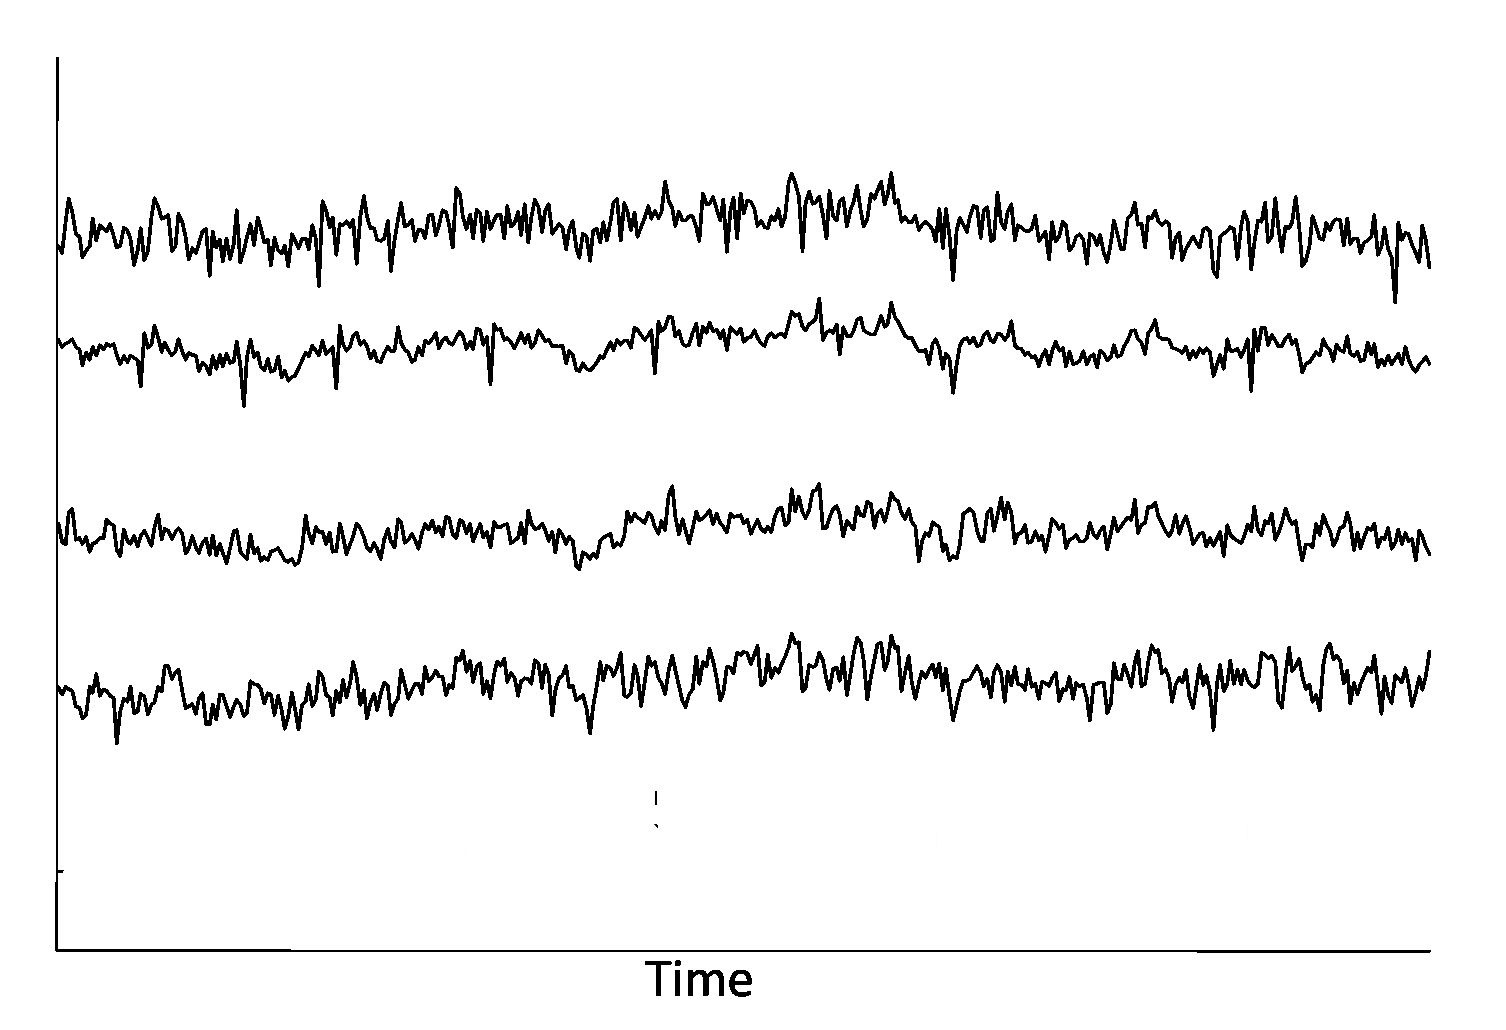
\includegraphics[height=.6\textheight]{multivariate_eeg}\\[1em]%
            \overimg{7}{meg_1}{8}{meg_dict}
        
        \textcolor{gray}{[{\color{linkcolor} NeurIPS 2018; ICASSP 2019}; article en préparation]}\\
        
%        \begin{itemize}
%            \item 1 article soumis en conférence,
%            \item 2 articles de journaux en cours de rédaction,
%            \item Un projet de partenariat en discussion avec B. Olshaussen (Berkeley).
%        \end{itemize}
    }
    \only<1-2>{
        \begin{itemize}
            \item Analyse de signaux de marche pour l'évaluation de l'équilibre.\\[1em]
        \end{itemize}
%        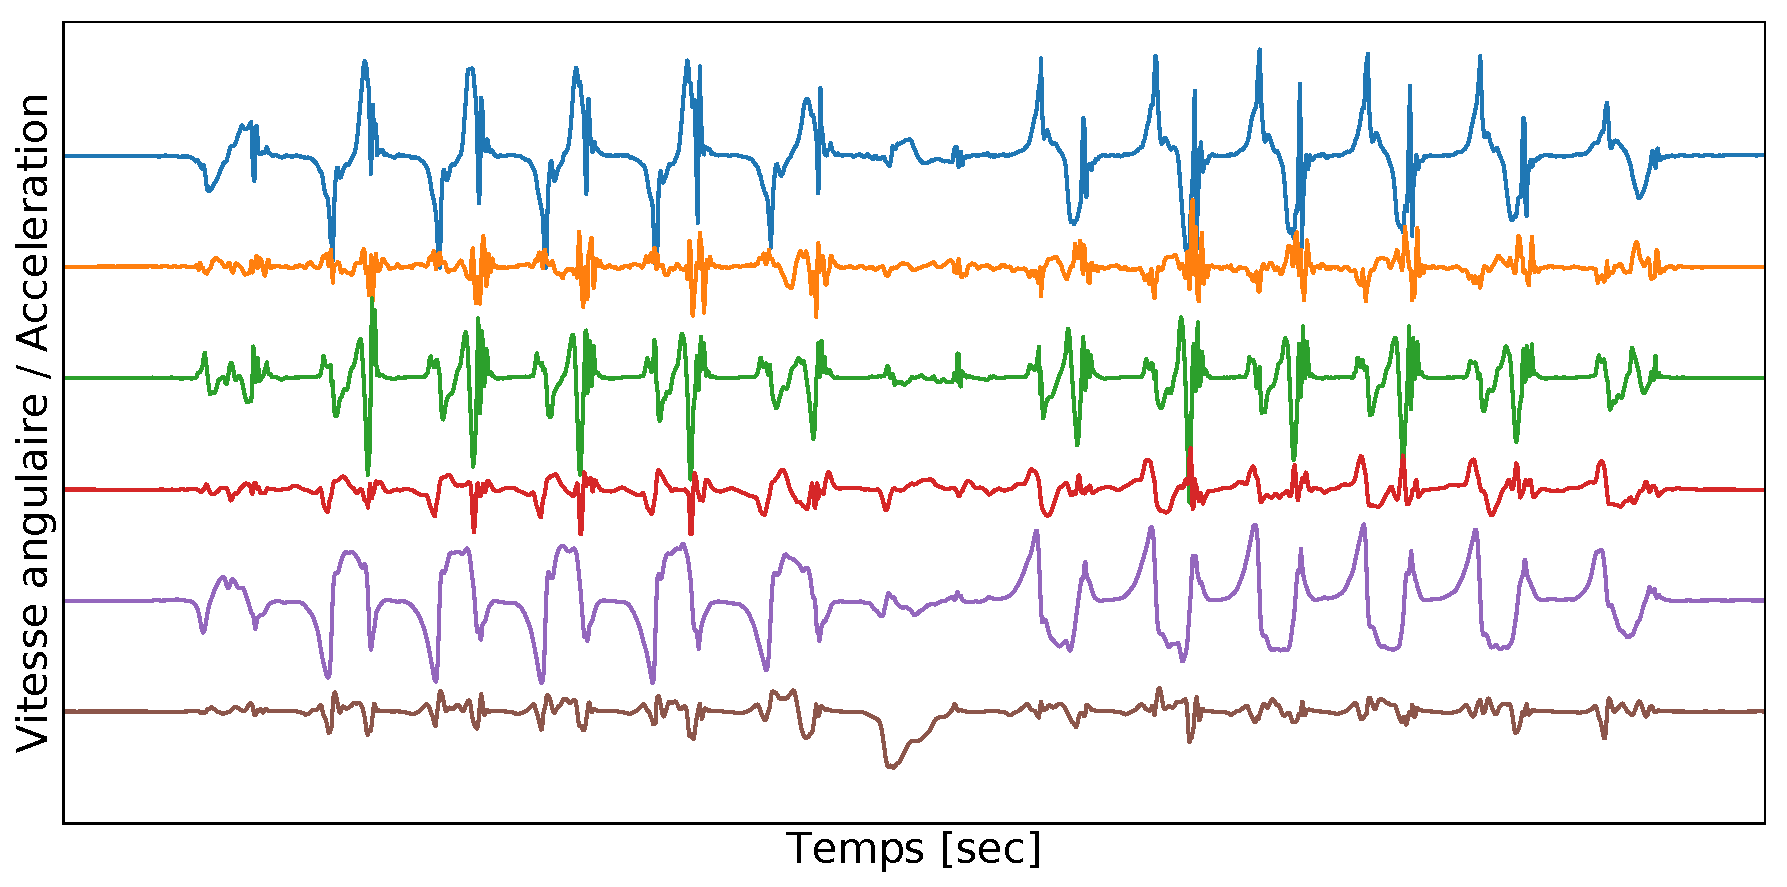
\includegraphics[height=.6\textheight]{accelero}\\[1em]%
        \overimg{1}{accelero}{2}{accelero_dict}
        
        {\color{gray}[{\color{linkcolor} PLoS ONE 2016; Sensors 2018}; Brevet 2015]}\\
        
%        \begin{itemize}
%            \item Un brevet déposé et en cours d'exploitation,
%            \item
%            \item En cours avec le laboratoire Cognac-G
%        \end{itemize}
    }
    \only<3-4>{
        \begin{itemize}
            \item Caractérisation de mouvements oculaires pathologiques.\\[1em]
        \end{itemize}
%        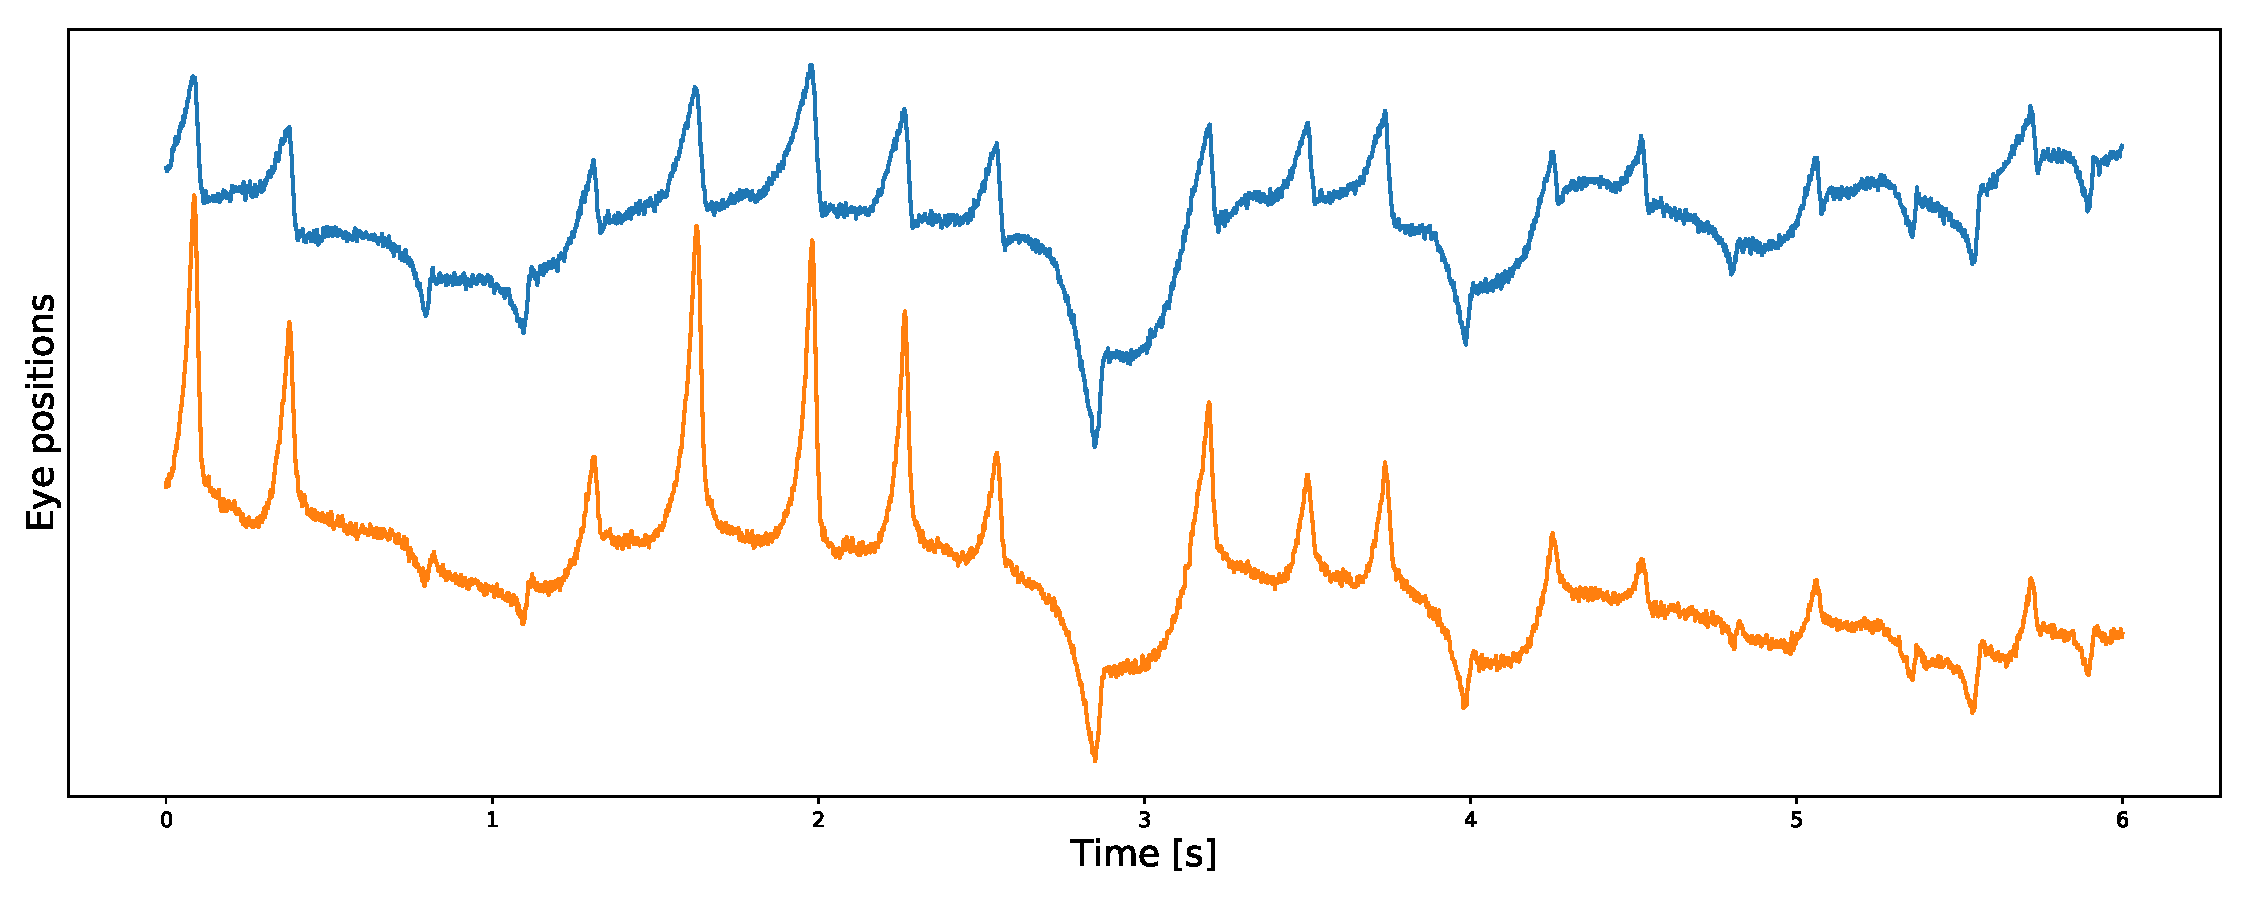
\includegraphics[height=.6\textheight]{oculo}\\[1em]%

        \overimg{3}{oculo}{4}{oculo_dict}
        \textcolor{gray}{[{\color{linkcolor} Plusieurs soumissions en cours}; stagiaire M2]}\\
    }
%    \only<4>{
%        \begin{itemize}
%            \item Comptage de cellules dans les images biologiques.\\[1em]
%        \end{itemize}
%        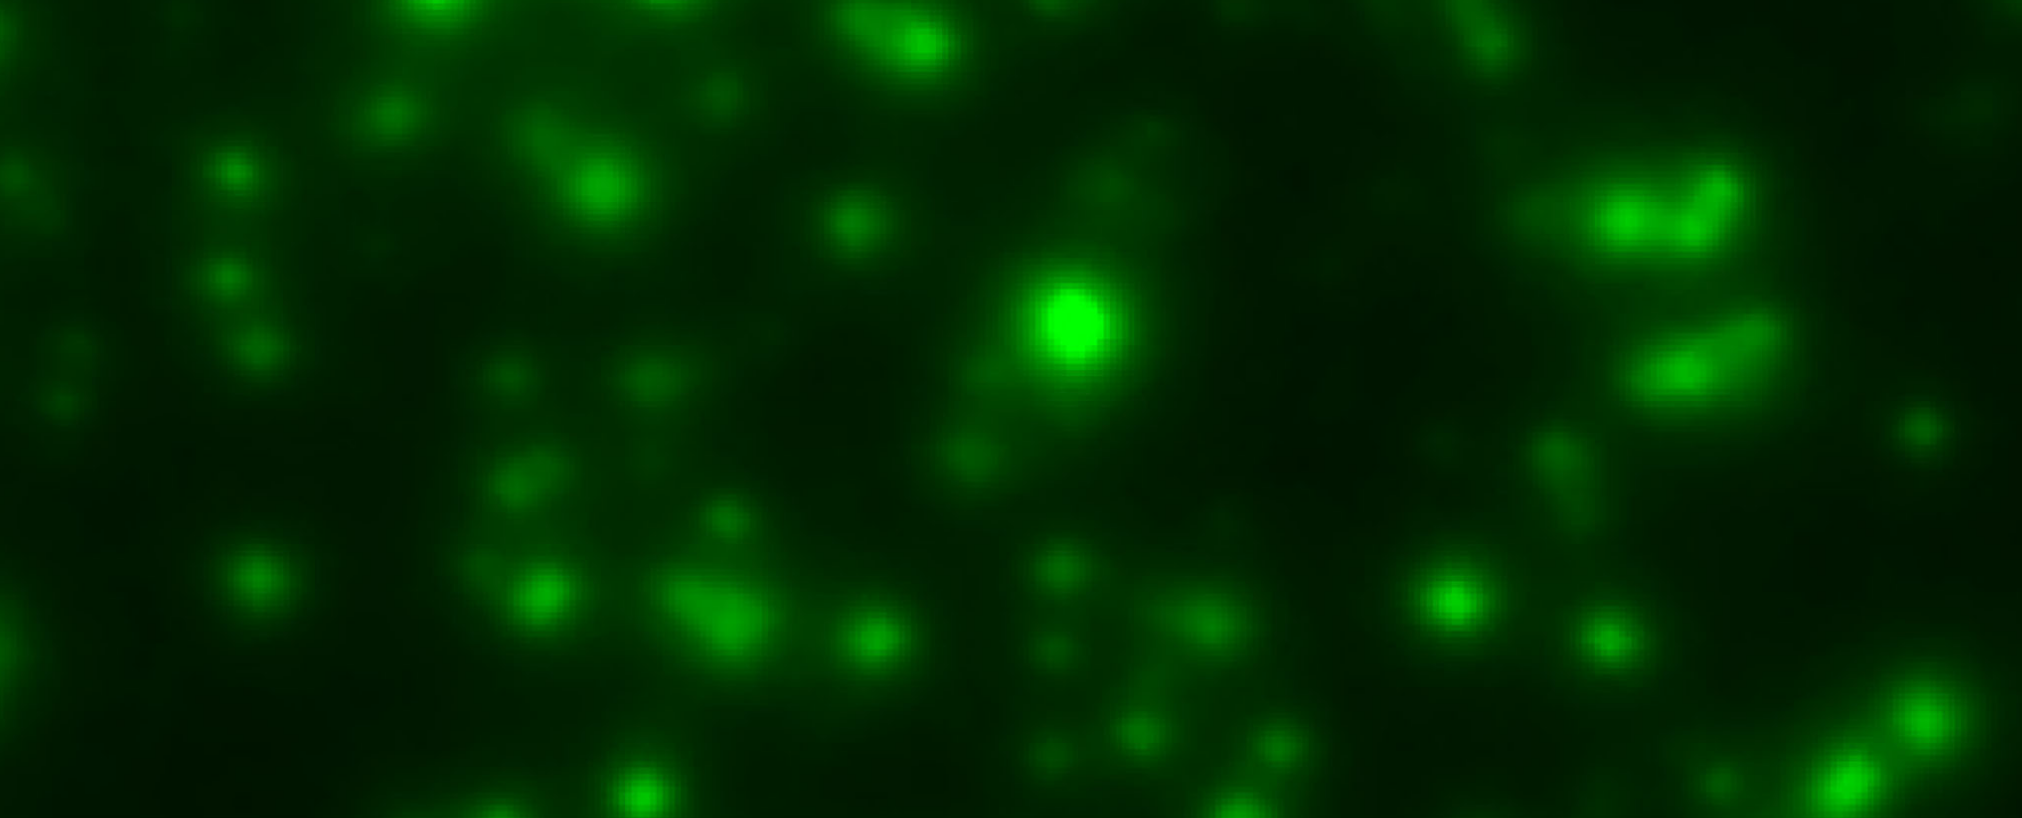
\includegraphics[height=.4\textheight]{fluospot}\\[1em]%
%        
%        [{\color{linkcolor}del Aguila Pla et al. 2018, IEEE TSP};
%        \citealt{Yellin2017}{\color{linkcolor}, ISBI}]\\
%    }
    \only<5-6>{
        \begin{itemize}
            \item Comptage d'objet astronomiques dans des images de telescope.\\[1em]
        \end{itemize}
        \overimg{5}{Hubble}{6}{Hubble_dict}    
        
        {\centering\textcolor{gray}{[{\color{linkcolor}preprint 2019}]}\\}
    }
}



\end{frame}

\begin{frame}[t]{Structure locale des signaux}
    \vskip1.5em
    \centering
    \only<1>{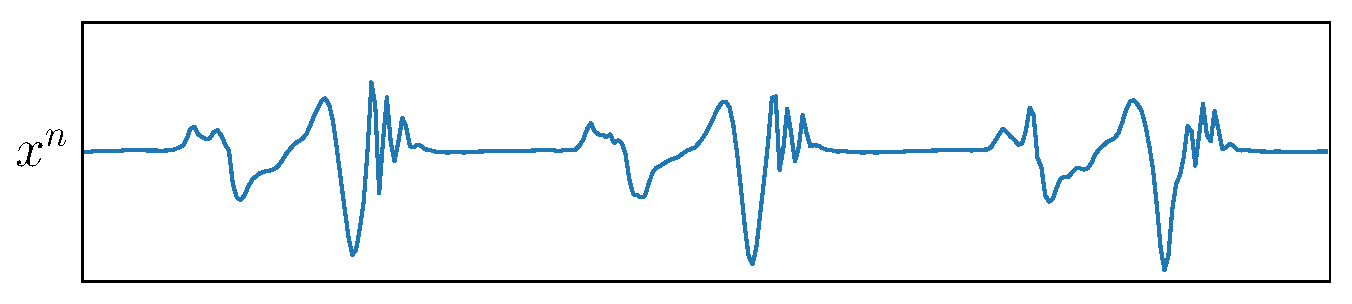
\includegraphics[width=\textwidth]{intro_csc_0}}%
    \only<2>{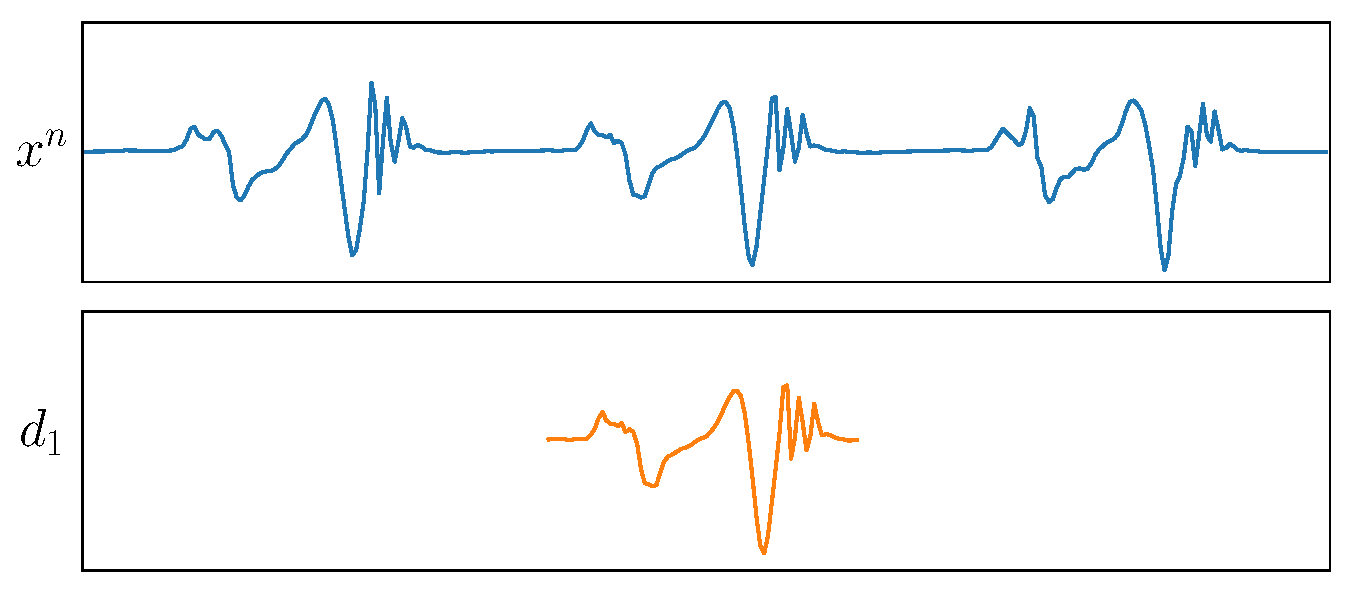
\includegraphics[width=\textwidth]{intro_csc_1}}%
    \only<3>{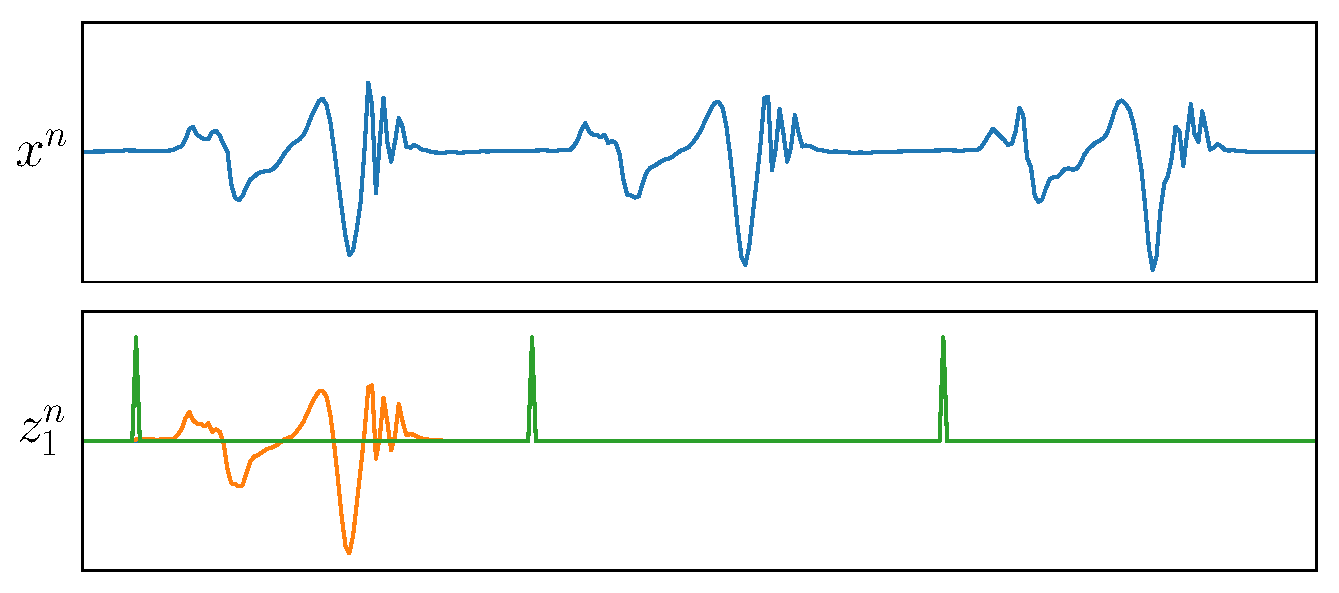
\includegraphics[width=\textwidth]{intro_csc_2}}%
    \only<4>{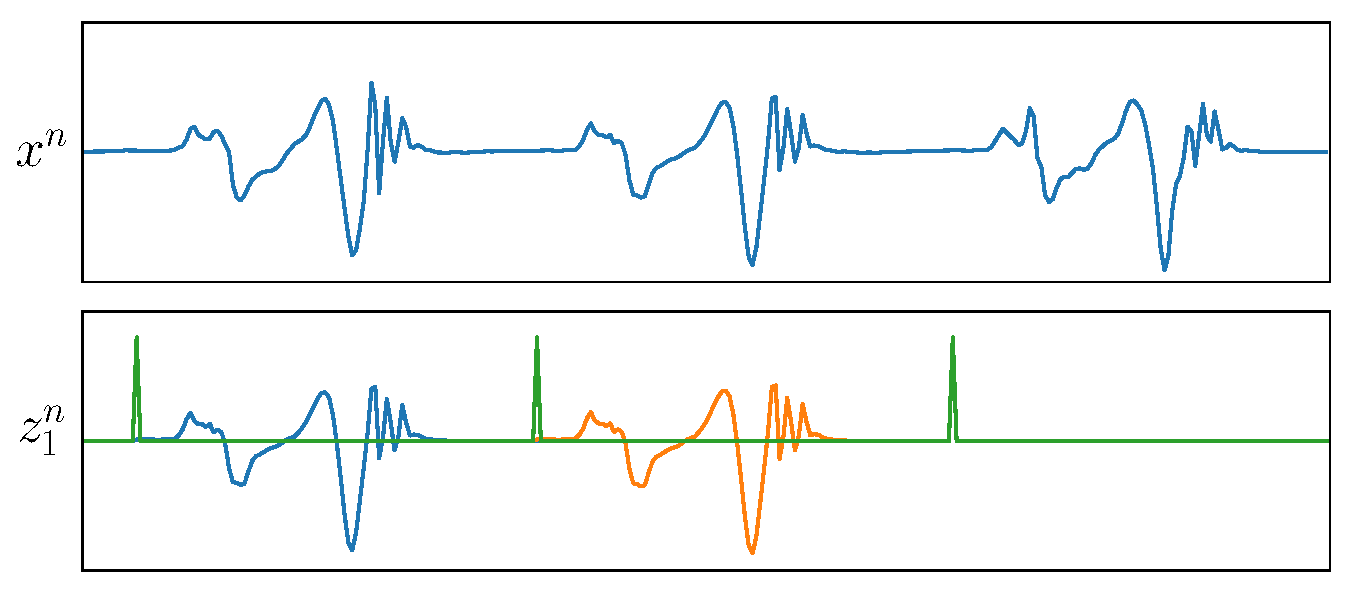
\includegraphics[width=\textwidth]{intro_csc_3}}%
    \only<5>{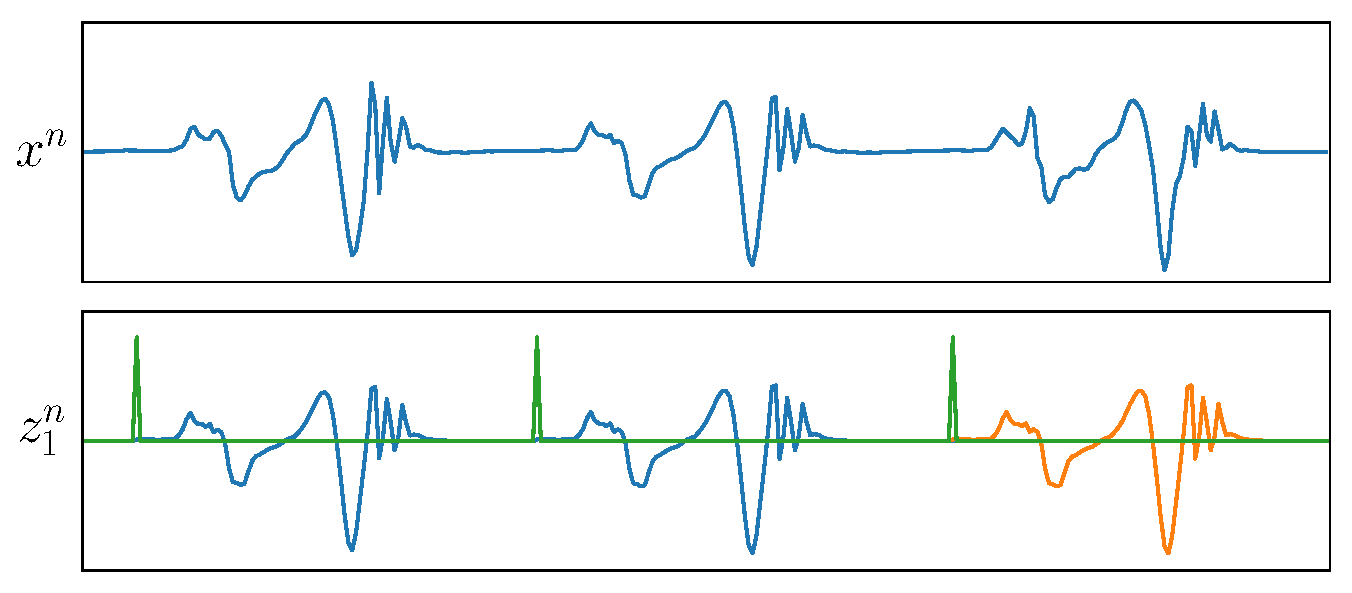
\includegraphics[width=\textwidth]{intro_csc_4}}%
    \only<6->{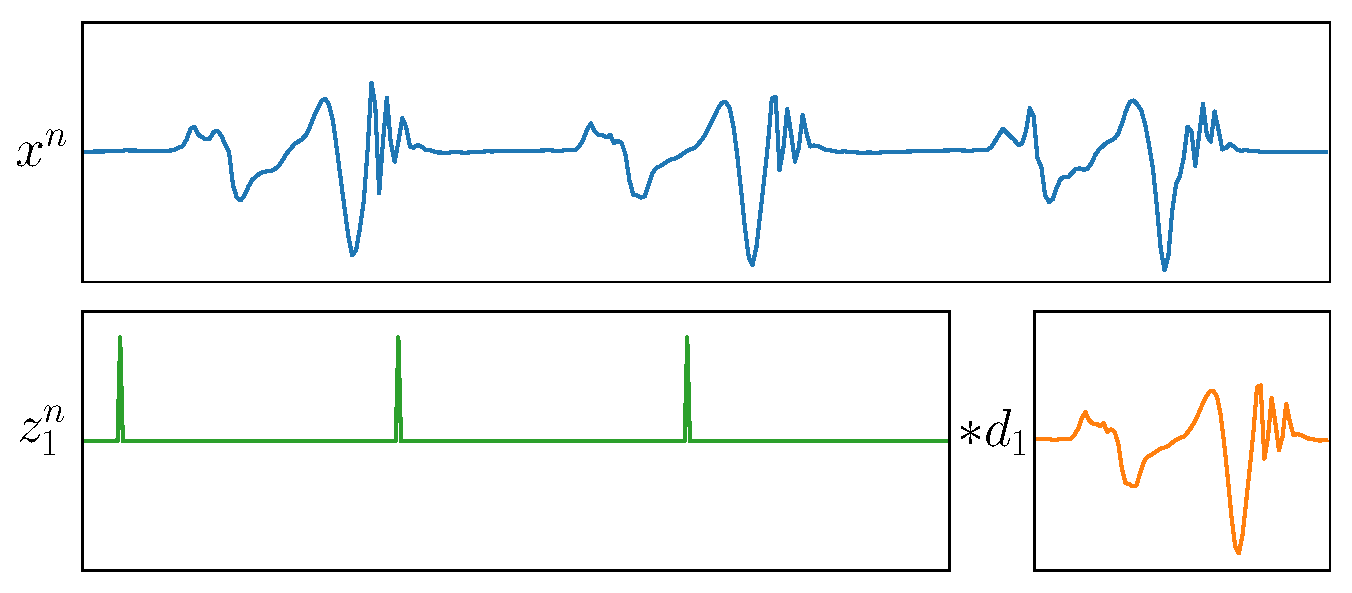
\includegraphics[width=\textwidth]{intro_csc_5}}%
    \vskip.2em
    \only<7>{%
        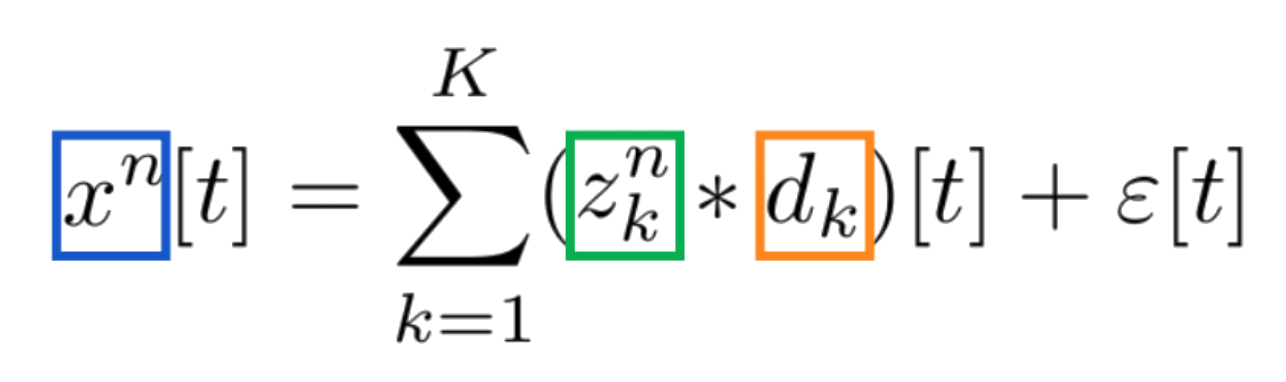
\includegraphics[width=.6\textwidth]{csc_explain_eq_color}
    }
    
 
\end{frame}

\begin{frame}{Challenges de l'apprentissage non-supervisé pour les signaux}


%\begin{columns}[c]
%    \column{1em}
%    %\rotatebox{90}{\Large Formation}
%    \column{.9\textwidth}
%    \begin{block}{Computationnel}
%        \myitem Parallélisation \hskip3em \myitem Structure du dictionnaire\\[.5em]
%        \keypoint{[{\color{linkcolor} ICML, 2018; preprint, 2019}]}
%    \end{block}
%\end{columns}
%
%
%\begin{columns}[c]
%\column{1em}
%\rotatebox{90}{\Large Axe 1}
%\column{.9\textwidth}
%\begin{block}{Modélisation}
%    \myitem Activations \hskip1em \myitem Motifs\\[.5em]
%    \keypoint{[{\color{linkcolor} NeurIPS, 2018; ICASSP, 2019}]}
%\end{block}
%\end{columns}
%
%
%\begin{columns}[c]
%    \column{1em}
%    \rotatebox{90}{\Large Axe 1}
%    \column{.9\textwidth}
%    \begin{block}{Théorique}
%        \myitem Évaluation des atomes \hskip1em \myitem Garanties d'estimation\\
%        \myitem Optimization globale\\[.5em]
%        \keypoint{[{\color{linkcolor} NeurIPS, 2018; ICASSP, 2019}]}
%    \end{block}
%\end{columns}


\begin{itemize}\itemsep1.5em
    \item \textbf{Computationnel:} passage à l'échelle pour les longs signaux,
    \begin{itemize}\itemsep.5em
        \item[$\bullet$] Parallélisation.%
                         \keypoint{ICML 2018; preprint 2019}
        \item[$\bullet$] Utilisation de la structure du dictionnaire.%
                         \keypoint{ICLR 2017}
    \end{itemize}

    \item \textbf{Modélisation:} incorporer de la connaissance de domaine,
    \begin{itemize}\itemsep.5em
        \item[$\bullet$] sur les activations.%
                         \keypoint{ICASSP 2019}
        \item[$\bullet$] sur les motifs.%
                         \keypoint{NeurIPS 2018}
    \end{itemize}

    \item \textbf{Théorique:} qualité des motifs appris.
    \begin{itemize}\itemsep.5em
        \item[$\bullet$] Évaluation statistique des atomes.
        \item[$\bullet$] Garantie algorithmique de convergence globale.
        \item[$\bullet$] Garantie de reconstruction des motifs.
        \item[$\bullet$] Lien avec l'apprentissage profond.%
                         \keypoint{ICLR 2017}
    \end{itemize}
\end{itemize}


\end{frame}


\begin{frame}[t]{DICOD: Optimisation distribuée pour le CDL%
              \keypoint{ICML, 2018}}
Résolution par descente de coordonnée gloutonne de\vskip-.5em
\[
    \argmin_{Z} \|X - D*Z\|_2^2 + \lambda \|Z\|_1
\]
\centering
\inputTikZ{.7}{DICOD}

\only<3->{
    \vskip1em
    \begin{block}{Propriété}
        \vskip.2em
        \myitem{} Algorithme asynchrone \hskip2em
        \myitem{} Communications locales efficaces\\[.3em]
        \myitem{} Converge vers le minimum global du problème\\[.3em]
        \myitem{} Passe à l'échelle super-linéairement
        \vskip.2em
    \end{block}
}
%
\only<4>{
    \vskip-1em
    \strongpoint{Extension pour signaux 2D}
    \vskip1em
    
\includegraphics[height=.8em]{github}~\textbf{DiCoDiLe}
    : \url{github.com/tommoral/dicodile}\\[1em]
}
\end{frame}



\begin{frame}{Application aux Neurosciences \keypoint{NeurIPS, 2018}}

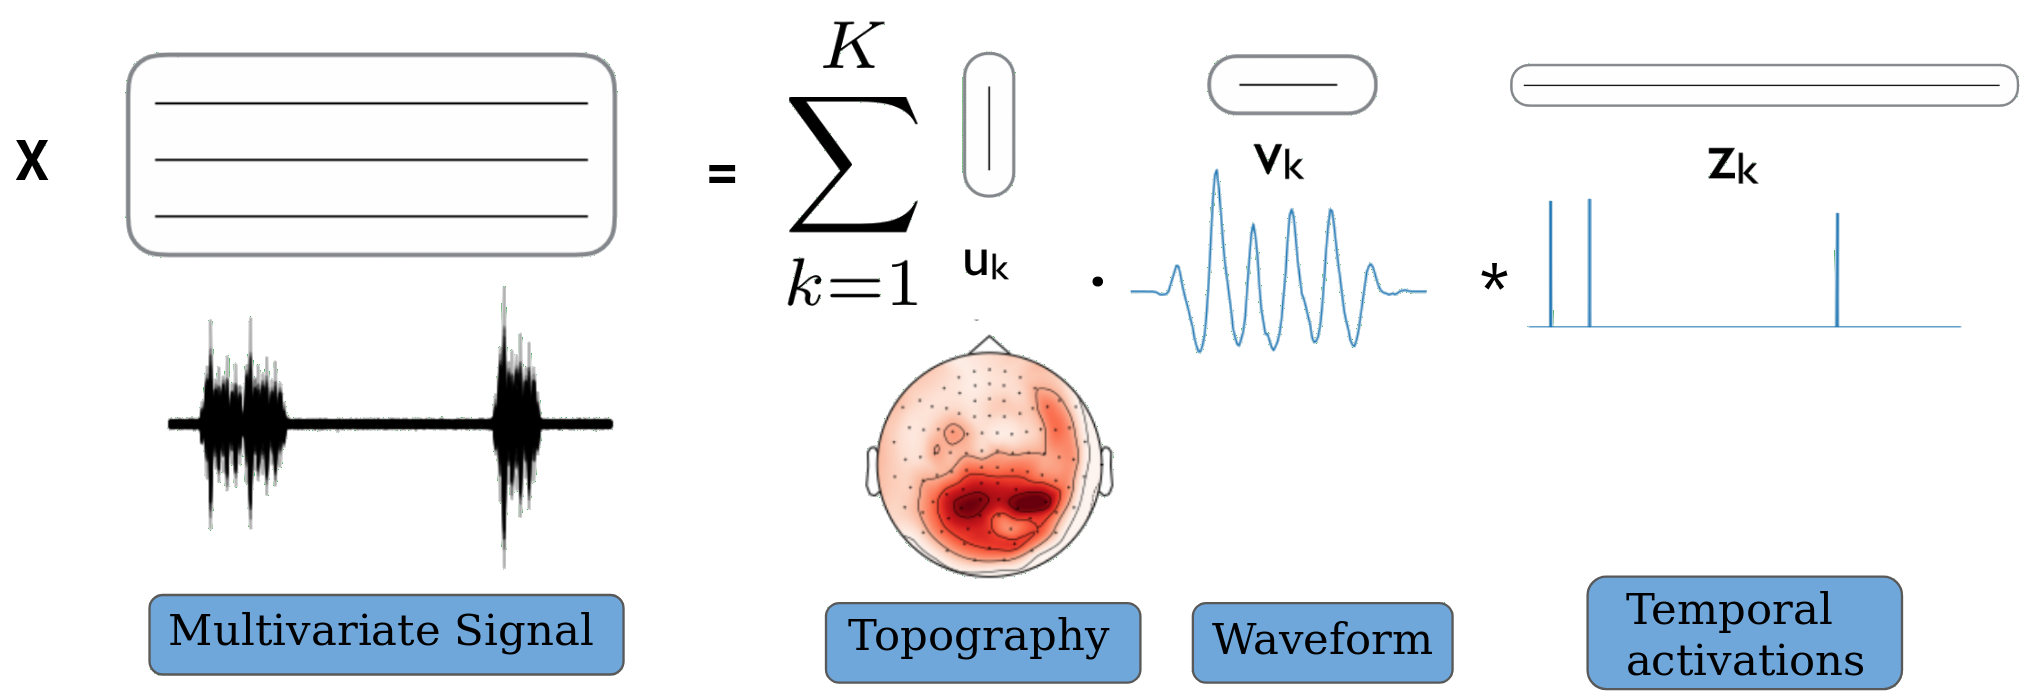
\includegraphics[width=\textwidth]{rank1}

\vskip1em
\begin{itemize}\itemsep.5em
    \item Modèle adapté à la physique des signaux MEG,
    \item Les atomes sont "explicables" (réponses évoquées, artefacts, \dots)
    \item Les activations capturent la latence dans les signaux MEG de tâches.
\end{itemize}
\vskip3em
\centering

\includegraphics[height=.8em]{github}~\textbf{alphacsc} : \url{alphacsc.github.io}\\[1em]
\end{frame}

\begin{frame}{Projet de recherche}


\begin{columns}[c]
\column{1em}
\rotatebox{90}{\Large Axe 1}
\column{.9\textwidth}
\begin{block}{Modélisation pour les signaux en neurosciences}
    \myitem Dépendance temporelle\hskip2em \myitem{}Modèle multi-échelles\\[.3em]
    \myitem Modélisation de l'activité neuronale\\[.3em]
\end{block}
\end{columns}
%
\vskip1em
\begin{columns}[c]
    \column{1em}
    \rotatebox{90}{\Large Axe 2}
    \column{.9\textwidth}
    \begin{block}{Analyse statistique des modèles convolutifs non-supervisés}
        \myitem Évaluation et reconstruction des atomes.\\[.3em]
        \myitem Convergence globale algorithmique.\\[.3em]
        \myitem Garantie de reconstruction des atomes.\\[.3em]
    \end{block}
\end{columns}
%
\vskip1em
\begin{columns}[c]
    \column{1em}
    \rotatebox{90}{\Large Axe 3}
    \column{.9\textwidth}
    \begin{block}{Apprentissage profond pour les problèmes inverses}
        \myitem Lien entre modèle convolutif et apprentissage profond.\\[.5em]
        \myitem Inversion rapide pour la localisation de source.\\[.5em]
    \end{block}
\end{columns}

\end{frame}



\begin{frame}[t]{Modélisation pour les signaux en neurosciences \keypoint{Axe 1}}
    \begin{columns}[T]%
        \column{2em}\vskip1em\rotatebox{90}{
            \begin{beamercolorbox}[rounded=true, wd=13em, center]{title}
                \large \bf Modélisation de l'activité
            \end{beamercolorbox}
        }
        \column{.45\textwidth}
        {\bf Processus ponctuel}\\[1.7em]
        {\centering
            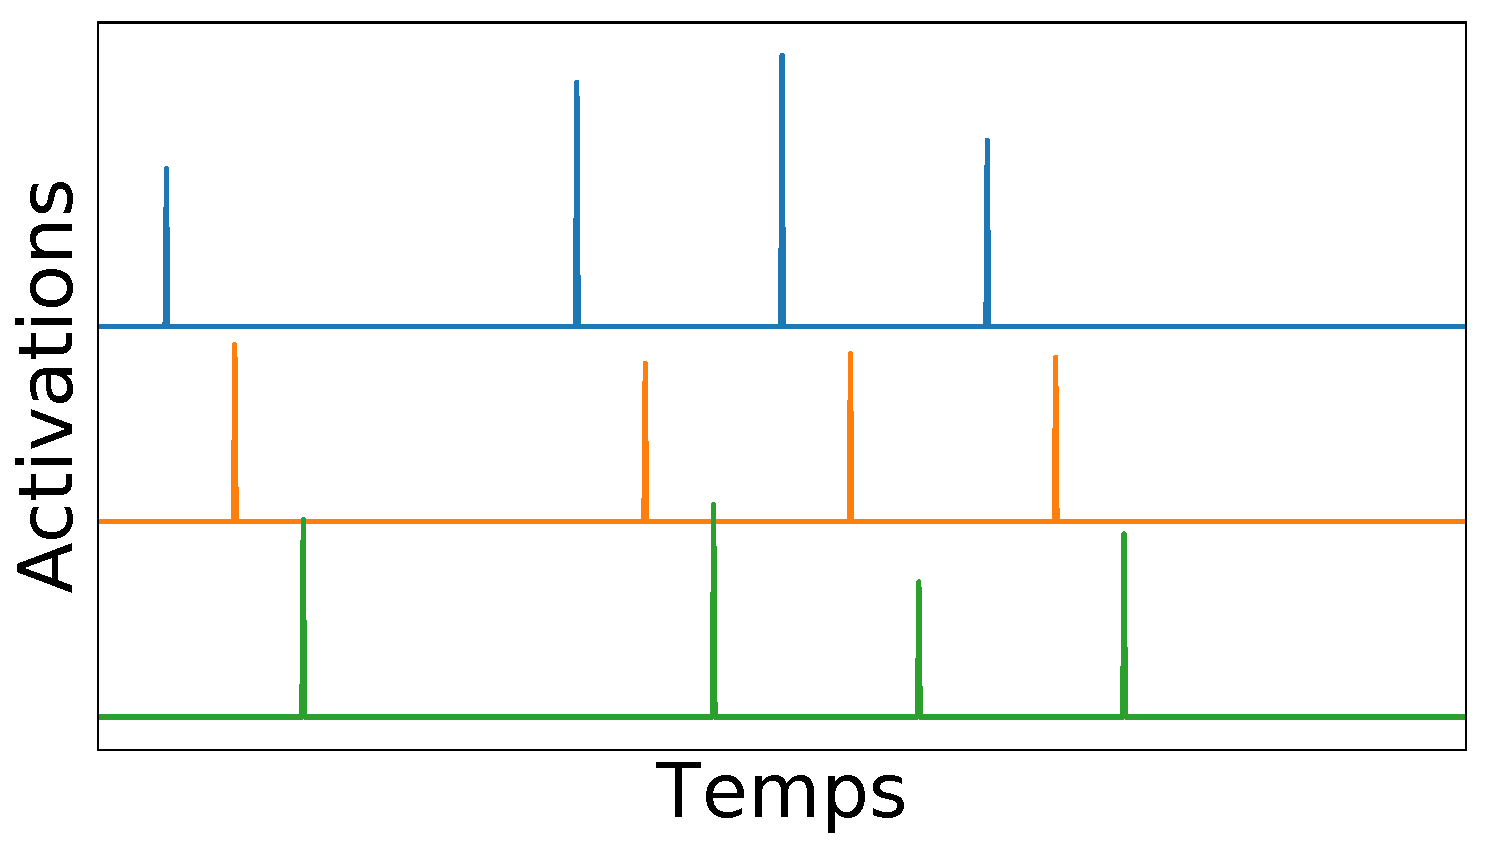
\includegraphics[width=.8\textwidth]{time_dependency}\\[1em]
        }
        

        \begin{itemize}
            \item Modéliser la dépendance entre les activations.
        \end{itemize}

    \column{2em}\vskip1em\rotatebox{90}{
        \begin{beamercolorbox}[rounded=true, wd=13em, center]{title}
            \large \bf Non-stationnarité
        \end{beamercolorbox}
    }
    \column{.45\textwidth}
    {\bf Apprentissage auto-supervisé}\\[.3em]
    {\centering
    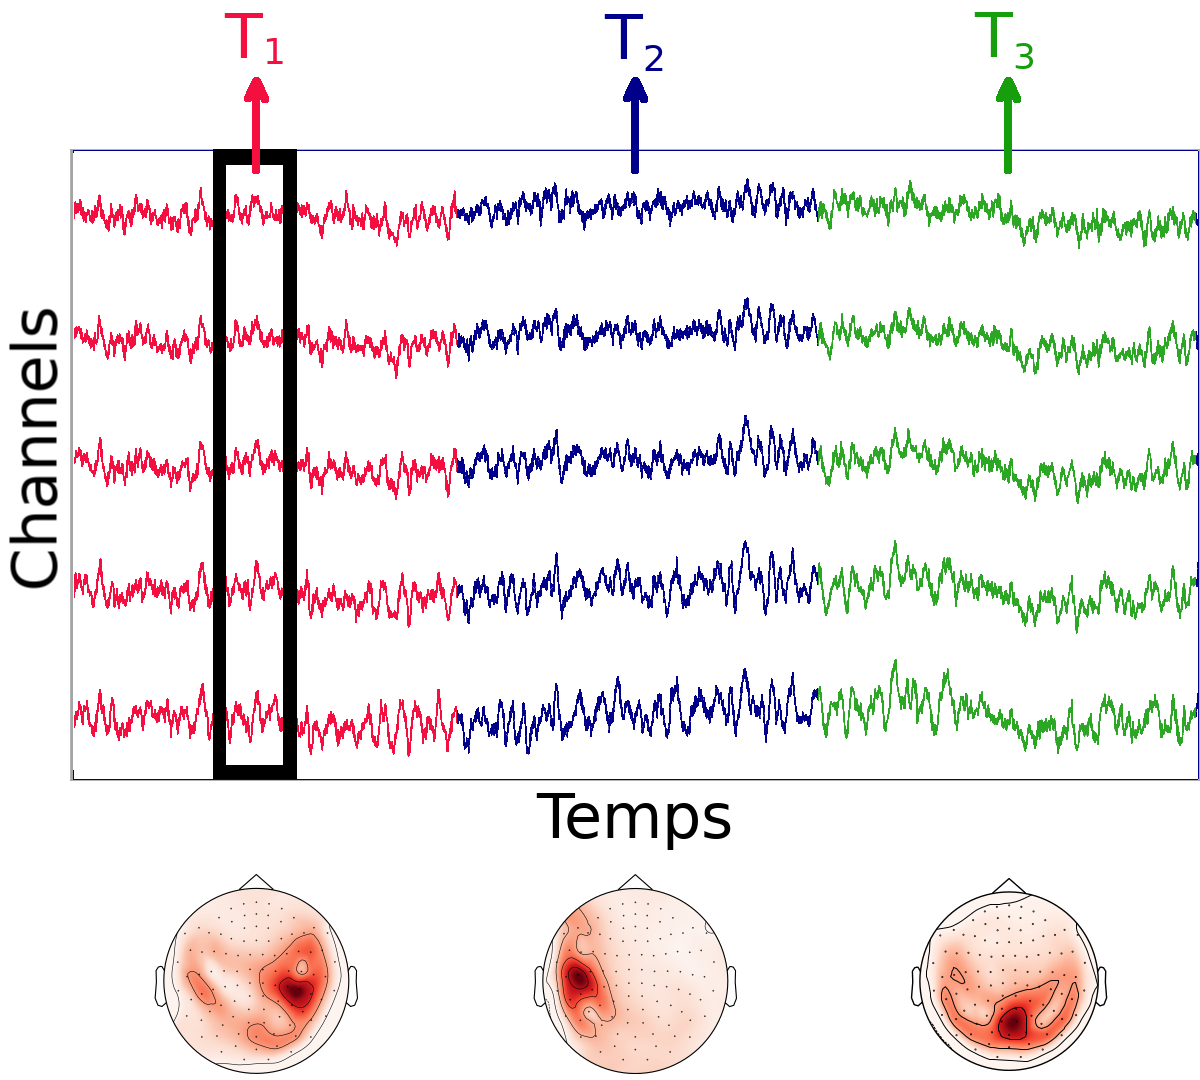
\includegraphics[width=.8\textwidth]{time_contrastive}\\[1em]
    }
    \begin{itemize}
        \item Atomes adaptés aux segments temporels.
    \end{itemize}
    \end{columns}
\vspace{0pt plus 1 filll}
{\centering \textbf{Prise en compte des dépendances temporelles}\\[1em]}
\end{frame}



\begin{frame}[t]{Analyse des modèles non-supervisés \keypoint{Axe 2}}
\begin{columns}[T]
    \column{2em}\vskip1em\rotatebox{90}{
        \begin{beamercolorbox}[rounded=true, wd=13em, center]{title}
            \large \bf Qualité des algorithmes
        \end{beamercolorbox}
    }
    \column{.45\textwidth}
    {\bf Garanties théoriques}\\[1em]
\begin{itemize}\itemsep.5em
    \item Il est possible de designer un algorithme avec une preuve de convergence globale si $K$ n'est pas fixé
    \item Analyse des propriétés de reconstruction théorique des motifs.
\end{itemize}
    
    
    \column{2em}\vskip1em\rotatebox{90}{
        \begin{beamercolorbox}[rounded=true, wd=13em, center]{title}
            \large \bf Évaluation des modèles
        \end{beamercolorbox}
    }
    \column{.45\textwidth}
    {\bf Auto-évaluation}\\[1em]
\begin{itemize}\itemsep.5em
    \item Apprendre un dictionnaire sur données d'entrainement.
    \item Encoder la moitié des canaux des données tests.
    \item Évaluer la reconstruction des autres canaux.
\end{itemize}
\end{columns}
\vspace{0pt plus 1 filll}
{\centering \textbf{Évaluation des modèles non-supervisés est un défi.}\\[1em]}
\end{frame}



\begin{frame}[t]{Apprentissage profond pour les problèmes inverses \keypoint{Axe 3}}
\begin{columns}[T]
    \column{2em}\vskip1em\rotatebox{90}{
        \begin{beamercolorbox}[rounded=true, wd=13em, center]{title}
            \large \bf Inversion rapide
        \end{beamercolorbox}
    }
    \column{.45\textwidth}
    {\bf Apprentissage profond}
        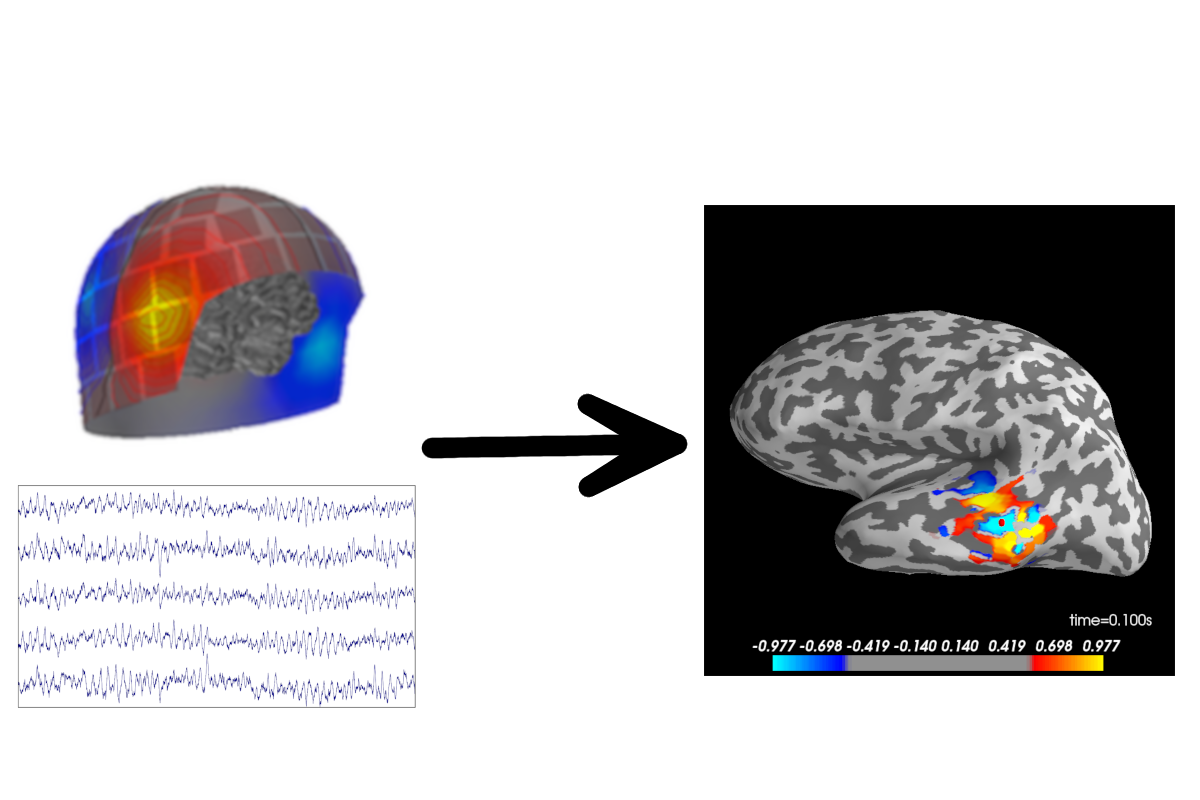
\includegraphics[width=\textwidth]{meg_inverse}

    \begin{itemize}\itemsep.5em
        \item Inversion du problème à partir de réseau de neuronne.
    \end{itemize}
    
    
    \column{2em}\vskip1em\rotatebox{90}{
        \begin{beamercolorbox}[rounded=true, wd=13em, center]{title}
            \large \bf Lien modèle convolutif
        \end{beamercolorbox}
    }
    \column{.45\textwidth}
    {\bf Algorithme d'optimsation appris}\\[1em]
    \begin{itemize}\itemsep.5em
        \item Extension du papier de ICLR 2017.
        \item Mécanisme d'accélération basé sur la structure de la matrice Hessienne.
        \item Lien avec l'analyse en composante principale parcimonieuse.
    \end{itemize}
\end{columns}
\vspace{0pt plus 1 filll}
%{\centering \textbf{Interpretabilité de l'apprentissage profond.}\\[1em]}
\end{frame}


%%===========================================================================
%\section{Conclusion}
%%===========================================================================
%
%\begin{frame}{Conclusion}
%    \textbf{Convolutional Dictionary Learning}
%    \begin{itemize}\itemsep.5em
%        \item Flexible pattern extraction technique,
%        \item Computationally tractable for more and more problems,
%        \item Some application are already beginning to emerge.
%    \end{itemize}
%    \vskip2em
%    \textbf{Challenges}
%    \begin{itemize}\itemsep.5em
%        \item Theoretical challenges remains (convergence, recoverability),
%        \item The evaluation (and thus the parameter choices) is still not clear,
%        \item Can give some insight for deep learning models?
%    \end{itemize}
%\end{frame}


\begin{frame}{Intégration dans l’équipe/collaborations}

\begin{columns}[c]
%    \column{1em}
%    \rotatebox{90}{}
    \column{.9\textwidth}
    \begin{beamercolorbox}[rounded=true, shadow=true]{title}
        \vskip-.1em%
        {\color{black} \bf Parietal}\\[.3em]
        \myitem{} Axe 1 : A. Gramfort, P. Ciuciu, D. Engemann\\[.3em]
        \myitem{} Axe 2 : B. Thirion, G. Varoquaux\\[.3em]
        \myitem{} Axe 3 : P. Ciuciu, A. Gramfort\\[.3em]
    \end{beamercolorbox}
\end{columns}


\vskip.5em
\begin{columns}[c]
%\column{1em}
\column{.9\textwidth}
\begin{beamercolorbox}[rounded=true, shadow=true]{title}
    \vskip-.1em%
    {\color{black}\bf National}\\[.3em]
    \myitem{} ENS Paris-Saclay (N. Vayatis) \hskip2em \myitem{} UP13 (L. Oudre)\\[.3em]
    \myitem{} Cognac-G (M. Robert, P.-P. Vidal).\\[.3em]
\end{beamercolorbox}
\end{columns}


\vskip.5em
\begin{columns}[c]
%\column{1em}
\column{.9\textwidth}
\begin{beamercolorbox}[rounded=true, shadow=true]{title}
    \vskip-.1em%
    {\color{black} \bf International:}\\[.3em]
    \myitem{} Berkeley (B. Olshausen)\\[.3em]
    \myitem{} NYU (J. Bruna).\\[.3em]
\end{beamercolorbox}
\end{columns}


\end{frame}


\begin{frame}[t]{Synthèse personnelle}%
\setlength{\parskip}{0em}
%
\begin{columns}[c]
    \column{1em}
    %\rotatebox{90}{\bf \large Parcours}%
    \column{.9\textwidth}%
    \begin{beamercolorbox}[rounded=true, shadow=true]{title}%
    {\large \bf \color{black} Parcours}\\
    2010-2014: X \hskip6em 2013-2014: Telecom ParisTech - MVA\\
    2014-2017: ENS Cachan \hskip1.4em 2018-2019: INRIA -- Parietal
\end{beamercolorbox}
\end{columns}%
%
\vskip1em
\begin{columns}[c]
    \column{1em}
    \rotatebox{90}{\large \bf Optim}
    \column{.9\textwidth}%
    \begin{beamercolorbox}[rounded=true, shadow=true]{title}
        Optimisation distribuée \hskip2em Modélisation des signaux\\
        Lien apprentissage profond et optimisation\\
        \keypoint{3 actes de conférence}
\end{beamercolorbox}
\end{columns}
\vskip1em
\begin{columns}[c]
    \column{1em}
    \rotatebox{90}{\bf \large Données}
    \column{.9\textwidth}%
    \begin{beamercolorbox}[rounded=true, shadow=true]{title}
        Analyse de la marche \keypoint{2 articles de journaux}\\
        Analyse des mouvements oculaire \keypoint{3 articles soumis}\\
        Neurosciences \keypoint{2 actes de conférence, 1 article en préparation}\\
\end{beamercolorbox}
\end{columns}
\vskip.7em
\begin{columns}[c]
    \column{1em}
    \rotatebox{90}{\bf \large Logiciel}
    \column{.9\textwidth}%
    \begin{beamercolorbox}[rounded=true, shadow=true]{title}
        Calcul parallèle en Python\\
        Développeur pour 3 librairies \keypoint{joblib, loky, threadpoolctl}\\
        Contributeur pour 2 projets \keypoint{CPython, scikit-learn}\\
\end{beamercolorbox}
\end{columns}

\end{frame}


%\begin{frame}{Profile}
%\begin{columns}[T]
%    \column{.33\textwidth}
%    \textbf{Machine Learning}\\
%    
%    \begin{itemize}
%        \item Unsupervised pattern recognition, Optimization
%        \item 3 papers in major conferences
%        \item 
%    \end{itemize}
%    \column{.33\textwidth}
%    \textbf{Open-source Software}
%    \begin{itemize}
%        \item Parallel computing in python
%        \item Core-developer of joblib (parallel computation engine for scikit-learn)
%        \item Contributed to important OSS projects (python, scikit-learn, ...)
%    \end{itemize}
%    \column{.33\textwidth}
%    \textbf{Applications}
%    \begin{itemize}
%        \item Oculographic recordings
%        \item Equilibrium assessments
%        \item Neuroscience
%    \end{itemize}
%\end{columns}
%\end{frame}
%===========================================================================
% AUXILIARY SLIDES
%===========================================================================



%===========================================================================
\appendix
\section{Auxiliary Slides}
%===========================================================================


%===========================================================================
\subsection{Aux1}
%===========================================================================
%
%\begin{frame}{Auxillary slide 1}
%
%\end{frame}
%
%
%\begin{frame}{}
%\vskip2em
%{\centering
%    \usebeamercolor[fg]{title}
%    \usebeamerfont{title}
%    \Huge \bf Merci!\\[2em]}
%
%Code available online:\\[1em]
%
%%
\includegraphics[height=.8em]{github}~\textbf{LISTA} : github.com/tommoral/AdaptiveOptim\\[1em]
%
%
\includegraphics[height=.8em]{github}~\textbf{alphacsc} :  \url{alphacsc.github.io}\\[2em]
%
%Slides are on my web page:\\[1em]
%\hskip5em\includegraphics[height=.8em]{website} \url{tommoral.github.io}
%\hskip4em 
\includegraphics[height=.8em]{twitter} \href{https://twitter.com/tomamoral}{@tomamoral}
%
%
%\end{frame}
%

\end{document}
